\appendix{Capacitance Simulation}\label{app:sim}

Here we have simulation data for the air gap design.
The electric field over a cross section of the electrode floating in space in the steel case
is shown in \ref{fig:app_sim}. The static field strength is calculated for the 
two positions of the case top at no load and max load conditions. 
The relaxed gap is 457 $\mu$m. 
The inner electrode is 30 $\mu$m, and sits 125 $\mu$m above the case.
The difference in dielectric strength above and below the
electrode is ignored for this simulation. 
For the max load conditions, the total gap is 200 $\mu$m.

The simulation points are chosen from the previous load frame characterization data of the sensor case.
The simulation covers a 0.1 degree chunk of the entire ring sensor.
The results of the simulation indicate that the uncompressed sensor should have a capacitance of 0.7 pf per degree of electrode
and the fully compressed electrode should have a capacitiance of 1.8 pf per degree of electrode.
This suggests the capacitance could change by at least 2.5 times its inital value over the travel of the sensor.

\begin{figure}[ht]
\centering
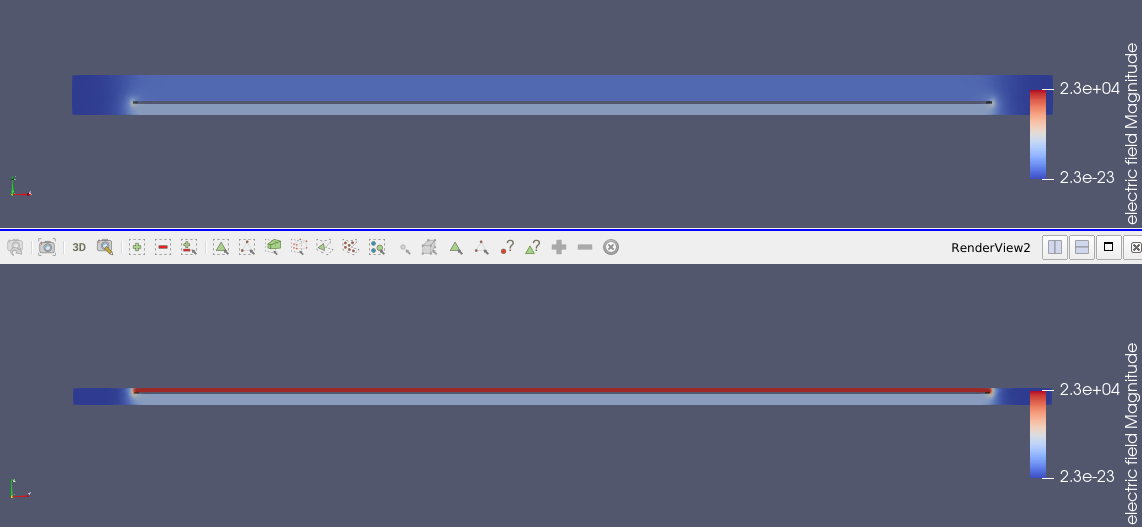
\includegraphics[width=0.7\textwidth]{app_sim.png}
\caption{
Simulation of electric field to determine capacitance properties of air gap design.
The top image shows the relaxed state of the sensor, with low electric field strength 
in the free space around the electrode.
When the air gap compresses, the electric field becomes much stronger and more concentrated,
this is measured as an increase in capacitance. Fringing effects appear to be minimal in this
simulation of the design.
}
\label{fig:app_sim}
\end{figure}
